% arara: pdflatex
% arara: pdflatex
% arara: pdflatex

% options:
% thesis=B bachelor's thesis
% thesis=M master's thesis
% czech thesis in Czech language
% slovak thesis in Slovak language
% english thesis in English language
% hidelinks remove colour boxes around hyperlinks

\documentclass[thesis=B,czech]{FITthesis}[2012/06/26]

\usepackage[utf8]{inputenc} % LaTeX source encoded as UTF-8
\usepackage[
	backend=biber
	,style=iso-numeric
	,sortlocale=cs_CZ
	,autolang=other
	,bibencoding=UTF8
]{biblatex}
\addbibresource{sources.bib}

\usepackage{graphicx} %graphics files inclusion
% \usepackage{amsmath} %advanced maths
% \usepackage{amssymb} %additional math symbols

\usepackage{dirtree} %directory tree visualisation

% % list of acronyms
% \usepackage[acronym,nonumberlist,toc,numberedsection=autolabel]{glossaries}
% \iflanguage{czech}{\renewcommand*{\acronymname}{Seznam pou{\v z}it{\' y}ch zkratek}}{}
% \makeglossaries

\newcommand{\tg}{\mathop{\mathrm{tg}}} %cesky tangens
\newcommand{\cotg}{\mathop{\mathrm{cotg}}} %cesky cotangens

% % % % % % % % % % % % % % % % % % % % % % % % % % % % % %
% ODTUD DAL VSE ZMENTE
% % % % % % % % % % % % % % % % % % % % % % % % % % % % % %

\department{Katedra softwarového inženýrství}
\title{Systém pro tvorbu a správu evolvabilních dokumentů}
\authorGN{Tomáš} %(křestní) jméno (jména) autora
\authorFN{Starý} %příjmení autora
\authorWithDegrees{Tomáš Starý} %jméno autora včetně současných akademických titulů
\author{Tomáš Starý} %jméno autora bez akademických titulů
\supervisor{Ing. Marek Suchánek}
\acknowledgements{Doplňte, máte-li komu a za co děkovat. V~opačném případě úplně odstraňte tento příkaz.}
\abstractCS{V~několika větách shrňte obsah a přínos této práce v~češtině. Po přečtení abstraktu by se čtenář měl mít čtenář dost informací pro rozhodnutí, zda chce Vaši práci číst.}
\abstractEN{Sem doplňte ekvivalent abstraktu Vaší práce v~angličtině.}
\placeForDeclarationOfAuthenticity{V~Praze}
\declarationOfAuthenticityOption{4} %volba Prohlášení (číslo 1-6)
\keywordsCS{Nahraďte seznamem klíčových slov v češtině oddělených čárkou.}
\keywordsEN{Nahraďte seznamem klíčových slov v angličtině oddělených čárkou.}
% \website{http://site.example/thesis} %volitelná URL práce, objeví se v tiráži - úplně odstraňte, nemáte-li URL práce

\begin{document}

% \newacronym{CVUT}{{\v C}VUT}{{\v C}esk{\' e} vysok{\' e} u{\v c}en{\' i} technick{\' e} v Praze}
% \newacronym{FIT}{FIT}{Fakulta informa{\v c}n{\' i}ch technologi{\' i}}

\begin{introduction}
	Pokud se chceme zabývat psaním dokumentů, je vhodné se nejdříve podívat do historie, na to kdy a jak se začaly psát první dokumenty, jak se psaní dokumentů
měnilo s tím jak se měnila vyspělost lidské civilizace.

V dnešní době má každý z nás možnost vytvořit dokument a sdílet jej s ostatními na celém světe a to všechno v rámci několika okamžiků. Toto ovšem nebylo
vždy možné. Podívejme se, jak jsme se jako lidstvo dostalo od~vyškrabávání znaků do~krunýřů až po dnešní psaní a sdílení dokumentu online.

\section{Od krunýřů ke knihtisku}

Základem každého dokumentu je písmo, písmo jako takové se prvně objevuje už v 7. tisíciletí před naším letopočtem a to v~Číně,
kde se našly kosterní pozůstatky a blízko nich i krunýře želv, na kterých se našlo první písmo. \cite{EarliestWriting} Toto je nejstarší doposud
nalezený artefakt obsahující písmo.

Písmo se o něco později také objevuje v Mezopotámii. Zde se objevuje klínové písmo, které přišlo jako zjednodušení pro piktogramy, které se používali
pro kontrolu obilí a dobytka. Společně s klínovým písmem se nezávysle na sobě rozvíjí písmo i na území starého Egypta, zde v podobě hieroglyfů. Tyto dvě
písma se pak rozšiřují po celém regionu, díky tomu roste v celém regionu efektivita ekonomiky a objevují se první historické záznamy
\cite{MesopotamiaHistory} a také první sepsané zákony.

V Mezopotámii se pro psaní klínového písma používaly hliněné destičky, kdežto ve starém Egyptě se používal papyrus. Papyrus se vyráběl ze stébel šáchoru
papírodárného a byl rozšířen po celém středomoří. Jeho výroba byla zapomenuta okolo roku 1100.

V Evropě se poté rozšiřuje používání papíru, který se k nám dostal z~Číny díky Arabům. Papír byl oproti pergamenům, které jsou vyráběny z~kůže, levnější
na výrobu, ale byl horší kvality, tudíž pro důležité dokumenty se používal pergamen. Do poloviny 15. století se ovšem stále většina dokumentů psala bez
použití sofistikované techniky, vše bylo stále opisováno ručně. To ovšem změnil Johan Gutenberg, který významně zdokonalil knihtisk, který se pak do
konce století rozšířil po celé Evropě. Knihtisk zde byl již dříve, ale Johan přišel s nápadem odlití jednotlivých písmen z~kovu, tím se zvýšila
jejich životnost a díky tomu se snížila cena celého tisku. Snížení ceny mělo za~následek rozšíření knih mezí více lidí a tím i zvednutí gramotnosti
obyvatelstva. \cite{ucebnice1}

\section{Průmyslová revoluce}

Ještě před příchodem průmyslové revoluce se objevují první pokusy o psací stroj a to již v roce 1714, kdy byl v Anglii patentován stroj
\uv{vyrážející písmenka na papír} \cite{FirstTypewriter}, ovšem s psacími stroji měl pramálo společného. O více než 100 let později se
objevuje první psací stroj, který přinesl rozložení kláves, které známe i z dnešních moderních počítačů. Toto rozložení bylo zavedeno kvůli
problémům se zasekáváním znaků při stisku více znaků po sobě, které se nacházely blízko sebe. Psací stroje zde s námi byly po většinu 20. století
a byly nahrazeny až počítači, ale o těch až později. Krom psacích strojů se s průmyslovou revolucí se také rozšiřují možnosti tisku, například roku 1799
si nechal N. L. Robert patentovat vynález stoje na výrobu papíru v tzv. \uv{nekonečném} pásu. \cite{Papir}

\section{Moderní technologie}

První počítače byly masivních rozměrů a zaměřeny pouze na určité početní operace, pro které byly sestrojené, jako například ENIAC, který byl za 2.
světové války na univerzitě v Pensylvánii, zde jej použivala americká armáda pro balistické výpočty. Tento počítač zabíral 185.81 $ m^2 $ plochy. \cite{historyComp} V roce
1947 přichází William Shockley, John Bardeen a Walter Brattain z Bell Laboratiories s vynálezem tranzistoru, pevného elektrického přepínače, který nepotřeboval
vakuum \cite{liveScience} (elektronky, které se používali do této doby, jej ke svému provozu potřebují). Jak je ale patrné z rozměrů takového stroje, je jasné,
že toto zařízení se rozšíření mezi masu lidí nedostálo, ovšem v 70. letech 20. století přicházejí první osobní počítače. Mezi lety 1974-1977 se na trhu objevují
první opravdové domácí počítače jako například Altair od Micro Instrumentation and Telemetry Systems (MITS). \cite{liveScience}

V roce 1976 Steve Jobs a Stephen Wozniak zakládají společnost Apple, jejich prvním produktem je Apple I, narozdíl od Altair měl tento počítač více paměti a levnější
procesor a monitor. O rok později začinají s produkcí Apple II, který nabízel barevnou obrazovku a možnost záznamu dat na přenosné médium, kazetu, která poté byla
nahrazena za disketu. Apple zárověň\linebreak s~vydáním Apple II vyzýval programátory, aby pro své počítače vytvářeli aplikace, díky tomu například vznikl první tabulkový program
nazývaný\linebreak VisiCalc~i~díky tomuto si Apple našel cestu nejen do domácností, ale i do firemního sektoru. \cite{liveScience}
\uv{První zpracovaní textu na počítači se stáva skutečností, když MicroPro International vydává WordStar.} \cite{liveScience}

\subsection{Software}

V dnešní době ale již existuje nepřeberné množství sofwaru na vytvoření a zpracování textu, uveďme si tedy ty nejznámnější i s~jejich krátkou historií. Začneme tedy
tím nejznámnějším, nejpoužívanějším a v dnešním době již braným jako standard, Word přišel na svět v roce 1983 \cite{word83}. Tato verze byla určena pro systém MS-DOS,
MS Office a s ním spojený Word jak jej známe dnes se ovšem objevil až v roce 1990, konkrétně 19. listopadu toho roku. S~jednotlivými verzemi se zlepšovalo grafické
rozhraní pro uživatele, s verzí 2016 přichází také optimalizace na mobilní zařízení a dotykové obrazovky. V roce 2011 je představen Office 365, online služba, ve
které je možné vytvářet a sdílet dokumenty odkudkoliv. \cite{word}

Neboť balíček Office je licencovaný firmou Microsoft a není možné jej používat bez licence, objevují se i open source řešení, mezi nejznámnější patří OpenOffice/LibreOffice,
jejich příběh začíná v roce 1999, kdy Sun Microsystems kupuje Star Division a mění název jejich produktu na OpenOffice.org, zárověň s tím vydávají kód k veřenjnému užití, open source,
každý si tedy může stáhnout kopii tohoto softwaru a užívat je jí volně. V roce 2009 kupuje Sun Microsystems firma Oracle, neboť měli někteří vývojáři z The Document Foundatiuon obavy,
co se stane s OpenOffice.org, vytvořili si vlastní odnož (fork) OpenOffice.org a začali ji dále rozvíjet pod názvem LibreOffice. Později díky tomuto vzniká i jednotný open source
formát pro sdílení dokumentů, Open Document Format (ODF). Díky vývojářům z Document Liberation Project je možné otevírat i ostatní formáty jako je .doc, .docx nebo importovat
soubory z Pages, což je Word v podání společnosti Apple. \cite{LibreHist}

\section{Shrnutí historie}

Jak je vidět, s postupujícím se technologickým rozvojem lidstva přicházelo i spoustu změn týkajících se tvoření dokumentů. Od dřívější víceméně ruční práce, která byla zahrnuta
ve všech aspektech se lidstvo dopracovalo do moderního pojetí, kdy není potřeba šířit dokumenty jejich opisováním a je\linebreak v~možnosti čím dál větší části lidstva vytvářet dokumenty,
které mohou být sdíleny po celém světe v rámci okamžiků díky internetu. Co se ovšem\linebreak nezměnilo, je přístup tvorby dokumentů, stále tvoříme dokument jako jeden celek, o~tom více
až v další kapitole.
\end{introduction}

\chapter{Analýza}
Historii psaní dokumentů jsme si popsali v minulé kapitole, nyní je čas popsat princip, kterým dokumenty vznikají. Vznik dokumentů totiž také prochází
vývojem, ale tento vývoj přichází až v poslední době s rozvojem informačních technologí. Tvorba dokumentů by se dala rozdělit na dva různé přístupy.
Jeden má za výsledek jeden soubor, který tvoří daný dokument a druhý pouze složí dokument z určitých částí.

Než si ovšem popíšeme tyto dva přístupy, je nutné se podívat jak vlastně dokument vzniká. Nejdříve je nutné vytvořit návrh neboli se také používá
označení draft. Tento draft je pouze základní obrys toho co by měl výsledný dokument obsahovat. Pokud se na dokumentu podílí vícero autorů, je
tento draft kontrolován každým z nich. Z draftu se potom začne rozvíjet výsledný dokument, který se po dopsání předává ke kontrole korektorům,
kde se kontroluje pravopis a stylistika. Po konečné kontrole díla autorem či autory je dílo předáno distributorovi. Celý tento postup
je znázorněn na grafu \ref{fig:linflow}

\begin{figure}[h]
    \centering
    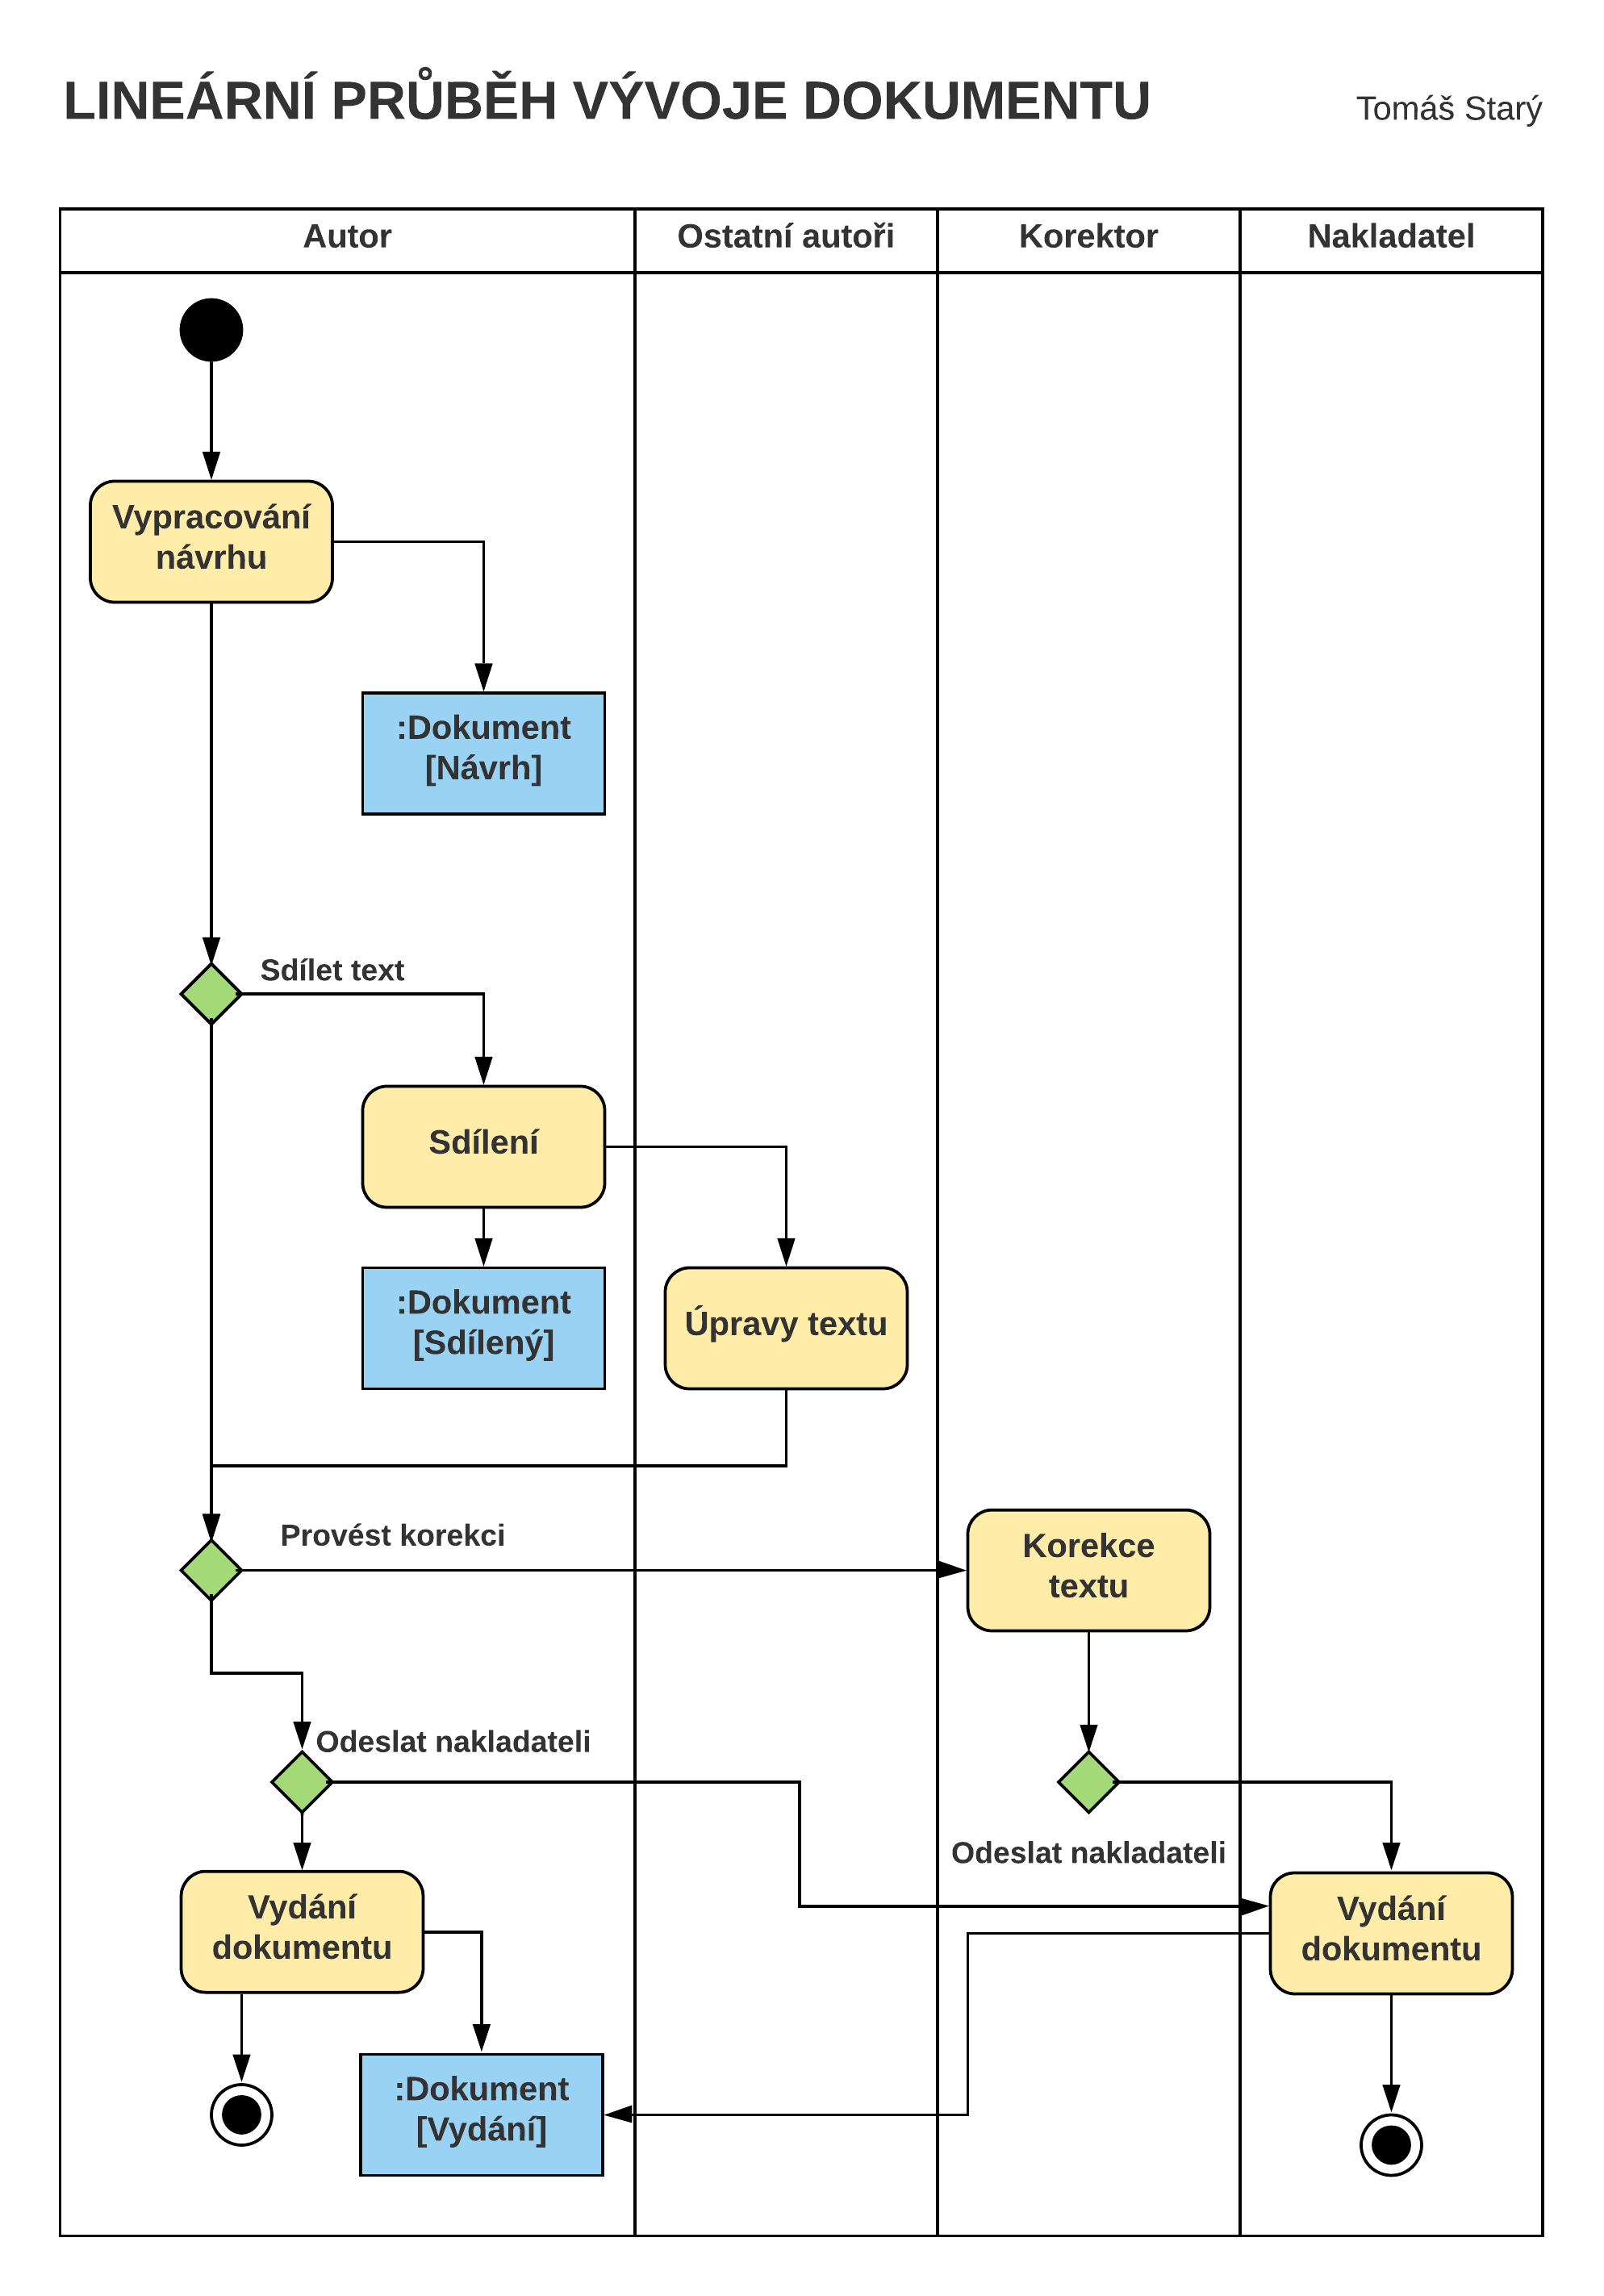
\includegraphics[width=\textwidth]{linearni_prubeh.png}
    \caption{Swimlines diagram}
    \label{fig:linflow}
\end{figure}

\section{Monolitický přístup}

Monolitickým přístupem je myšleno to, že jednotlivé dokumenty jsou jednotné celky, jeden dokument je jeden celek. Pro představu, pokud si vezmeme ku příkladu
Word, o kterém už zaznělo něco v kapitole o historii psaní dokumentů, vytvořením jednoho souboru s příponou .docx, jsme vytvořili jeden monolitický dokument, pokud jej
budeme chtít použít v jiném dokumentu, budeme muset obsah tohoto souboru zkopírovat do nového souboru. Tento nový soubor, který bude obsahovat i náš původní dokument,
pokud se ovšem něco změní v původním dokumentu, druhý dokument bude mít stále původní verzi. Toto poté přináší problémy, které byly již nastíněny v úvodu této práce.

\section{Modulární přístup}




\chapter{Realizace}

\begin{conclusion}
	%sem napište závěr Vaší práce
\end{conclusion}

\printbibliography
\appendix

\chapter{Seznam použitých zkratek}
% \printglossaries
\begin{description}
	\item[GUI] Graphical user interface
	\item[XML] Extensible markup language
\end{description}

\chapter{Obsah přiloženého CD}

%upravte podle skutecnosti

\begin{figure}
	\dirtree{%
		.1 readme.txt\DTcomment{stručný popis obsahu CD}.
		.1 exe\DTcomment{adresář se spustitelnou formou implementace}.
		.1 src.
		.2 impl\DTcomment{zdrojové kódy implementace}.
		.2 thesis\DTcomment{zdrojová forma práce ve formátu \LaTeX{}}.
		.1 text\DTcomment{text práce}.
		.2 thesis.pdf\DTcomment{text práce ve formátu PDF}.
		.2 thesis.ps\DTcomment{text práce ve formátu PS}.
	}
\end{figure}

\end{document}
